\documentclass[fleqn,10pt,serif,xcolor=svgnames,xcolor=table,aspectratio=169,handout]{beamer}
% \includeonlyframes{current}
%========================================
% Packages
%========================================

\usepackage[palatino]{mypackBeamer}
%========================================
% More Layout (Beamer Special)
%========================================

\DefineNamedColor{named}{mycol}{cmyk}{0.6,0.6,0,0}
% \DefineNamedColor{named}{mygray}{cmyk}{0.05,0.05,0.05,0.05}
% \DefineNamedColor{named}{mygraylight}{cmyk}{0.017,0.017,0.017,0.017}

\definecolor{signal1}{rgb}{0.69, 0.25, 0.21}
\definecolor{signal2}{rgb}{1.0, 0.66, 0.07}
\definecolor{signal3}{rgb}{0.39, 0.58, 0.93}
\definecolor{signal4}{rgb}{0.0, 0.4, 0.0}
\definecolor{firebrick}{rgb}{0.7, 0.13, 0.13}
\definecolor{themecolor}{rgb}{0.3, 0.36, 0.33} % feldgrau
\definecolor{darkgray}{rgb}{0.66, 0.66, 0.66}

% \usetheme[height=7mm]{Rochester}
%\usetheme{Warsaw}


\usecolortheme{dove}

% \useoutertheme[compress,subsection=false]{miniframes}

\usecolortheme[named=themecolor]{structure}

\setbeamercolor{title}{fg=themecolor}

% \setbeamercolor{lower separation line head}{bg=white}

%\setbeamercolor{structure}{fg=Brown}
%\setbeamercolor{normal text}{fg=Brown}
%\setbeamercolor{section in head/foot}{bg=gray!40}
%%\setbeamercolor{lower separation line head}{bg=black!40}
%\setbeamercolor*{frametitle}{fg=Black,bg=gray!40}
%\setbeamercolor*{block body}{fg=Brown,bg=gray!00}
%\setbeamercolor*{block title}{fg=Black,bg=gray!40}


% Switch of shadows of boxes
\setbeamertemplate{blocks}[default]

% Frame numbers in footer
\setbeamertemplate{footline}[frame number]

% See-through preview for uncovered
% \setbeamercovered{transparent}

% Switch off navigation panel at bottom right
\beamertemplatenavigationsymbolsempty

% Change Style for itemize markers
% Options are ball, circle, rectangle and default (=triangle)
\setbeamertemplate{items}[circle]



\setcounter{tocdepth}{1}

% Use bullets in enumerates and TOC
\setbeamertemplate{enumerate item}[circle]

% Set color for enumerate/TOC bullets to white
\setbeamercolor*{item projected}{fg=themecolor,bg=gray!00}

\setbeamercolor*{author}{fg=gray!80}

\setbeamerfont*{block title}{size=\normalsize}
\setbeamerfont*{title}{size=\huge}
\setbeamerfont*{subtitle}{size=\large}

% \newcommand{\mygray}[1]{{\color{gray}{#1}}}
% \newcommand{\mycol}[1]{{\color{mycol}{#1}}}

\newcommand{\mycomment}[1]{\hfill {\mygray{#1}}}
\newcommand{\mycom}[1]{\hfill {\mygray{[#1]}}}

\newcommand{\slideFN}[1]{%
  \begin{textblock*}{\paperwidth}(0pt,1.05\textheight)
    \hfill \footnotesize{\mygray{#1}} \hspace{.5em}
  \end{textblock*}}

\newcommand{\pictureslide}[2][current]{
\usebackgroundtemplate{\includegraphics[width=\paperwidth]{#2}}%
\begin{frame}[label=#1]

\end{frame}
}
% code below makes it possible to turn inclusion of frames
% into 'miniframes' off and on with commands:
% \miniframeson and \miniframesoff
% from: http://tex.stackexchange.com/questions/37127/how-to-remove-some-pages-from-the-navigation-bullets-in-beamer

\makeatletter
\let\beamer@writeslidentry@miniframeson=\beamer@writeslidentry
\def\beamer@writeslidentry@miniframesoff{%
  \expandafter\beamer@ifempty\expandafter{\beamer@framestartpage}{}% does not happen normally
  {%else
    % removed \addtocontents commands
    \clearpage\beamer@notesactions%
  }
}
\newcommand*{\miniframeson}{\let\beamer@writeslidentry=\beamer@writeslidentry@miniframeson}
\newcommand*{\miniframesoff}{\let\beamer@writeslidentry=\beamer@writeslidentry@miniframesoff}
\makeatother

\setbeamertemplate{bibliography item}{}

\usepackage{mycommands}
\usepackage{array}
\usepackage[absolute,overlay]{textpos}

\usepackage{ulem}

% \usetheme[]{boxes}

%========================================
% Commands
%========================================

\newcommand{\mycol}[1]{{\textcolor{mycol}{#1}}}
\renewcommand{\markdef}[1]{\mycol{#1}}
\newcommand{\mygray}[1]{\textcolor{gray}{#1}}

\renewcommand{\slideFN}[1]{%
  \begin{textblock*}{\paperwidth}(0pt,0.95\textheight)
    \hfill \footnotesize{\mygray{#1}} \hspace{.5em}
  \end{textblock*}}

%========================================
% Document
%========================================

\title{Sets, elements \& cardinality}
\subtitle{Methods: Logic, Part 1a}

\author{Michael Franke}
\date{}


%--------------------------------------


\begin{document}

% --- Horizontal Space Fix ----

\abovedisplayskip=3pt
\abovedisplayshortskip=3pt

\belowdisplayskip=3pt
\belowdisplayshortskip=3pt

\begin{frame}
  \maketitle
\end{frame}

\begin{frame}
  \frametitle{Content covered}

  \begin{itemize}
    \item basics notions of na\"{i}ve set theory:
            \begin{itemize}
              \item universe
              \item element
              \item set
              \item membership
              \item cardinality
            \end{itemize}
    \item ways of describing or defining sets
  \end{itemize}
\end{frame}

\begin{frame}
  \frametitle{Universe}
  \framesubtitle{All the stuff we care about}

  \begin{center}
    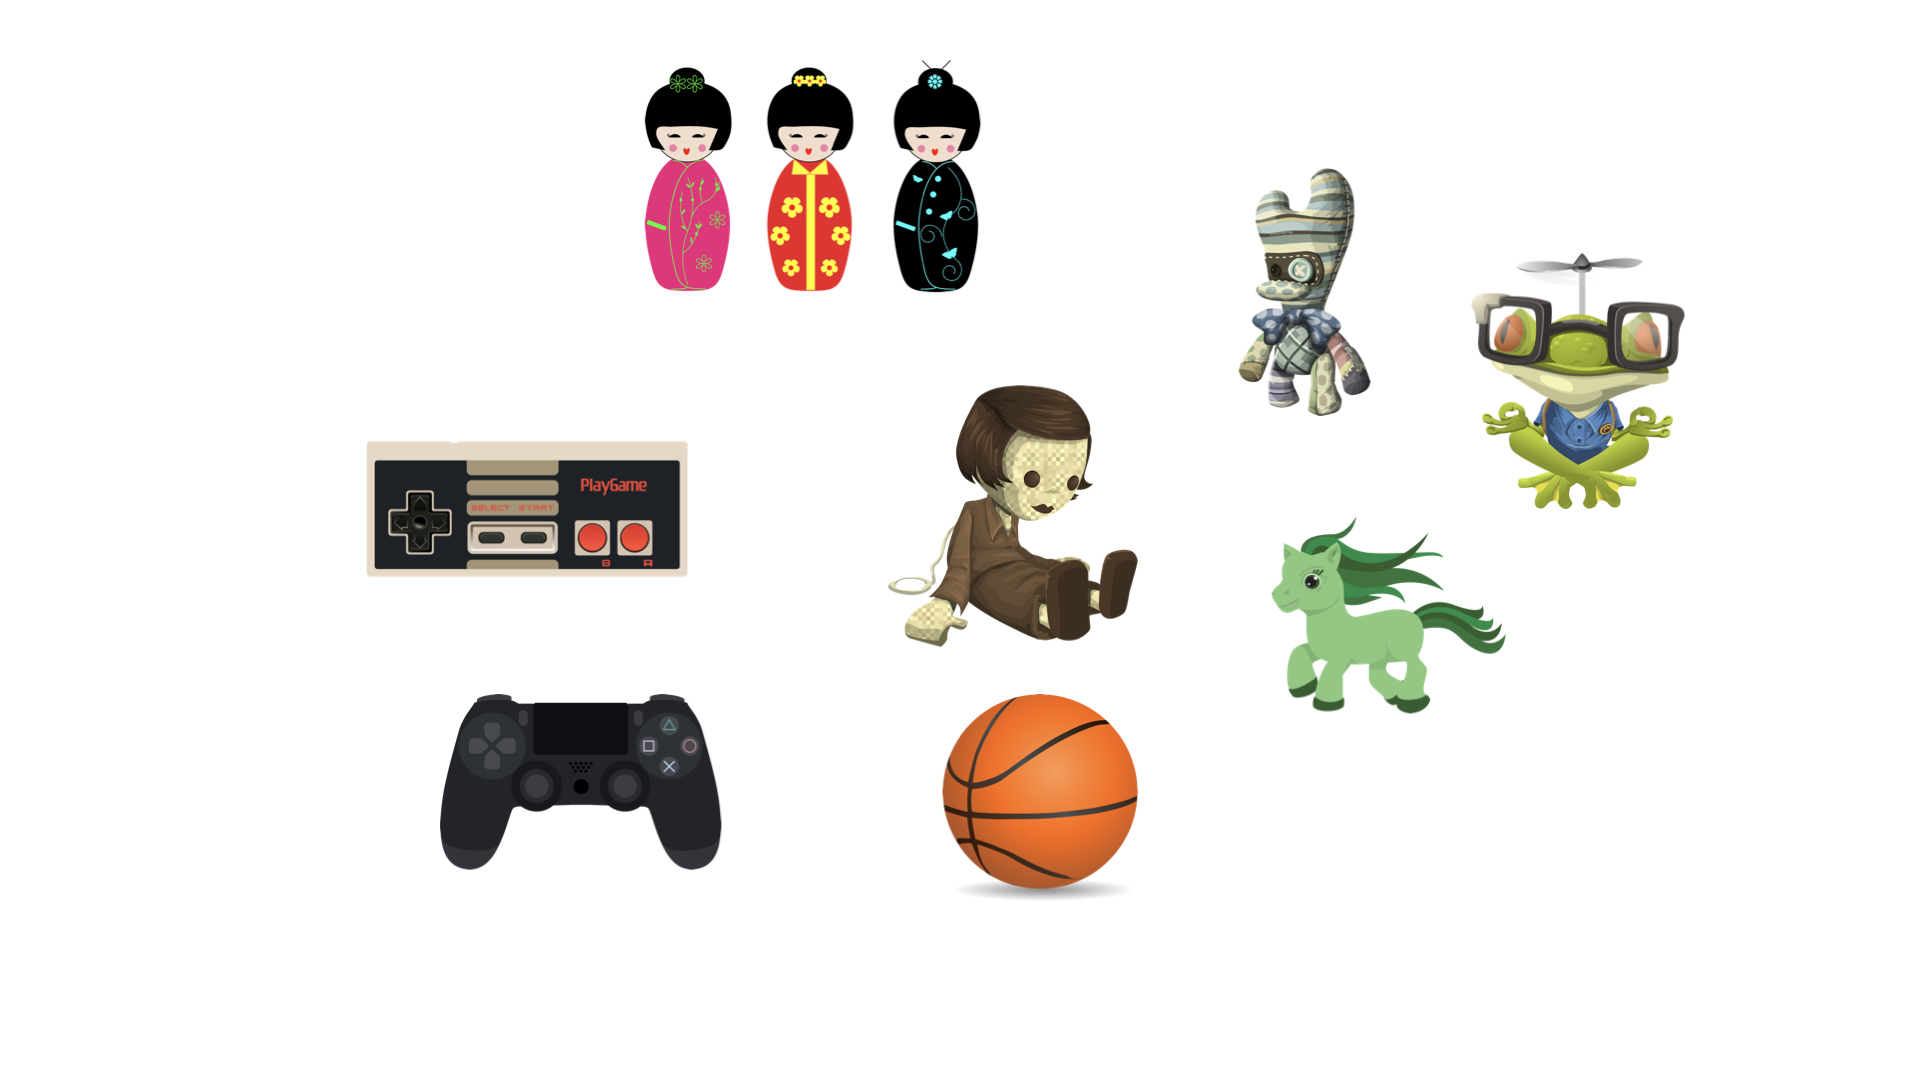
\includegraphics[width=\textwidth]{01a-sets-elements-cardinality/01a-sets-elements-cardinality-001.jpeg}
  \end{center}
\end{frame}

\begin{frame}
  \frametitle{Set}
  \framesubtitle{A collection of elements}

  \begin{center}
    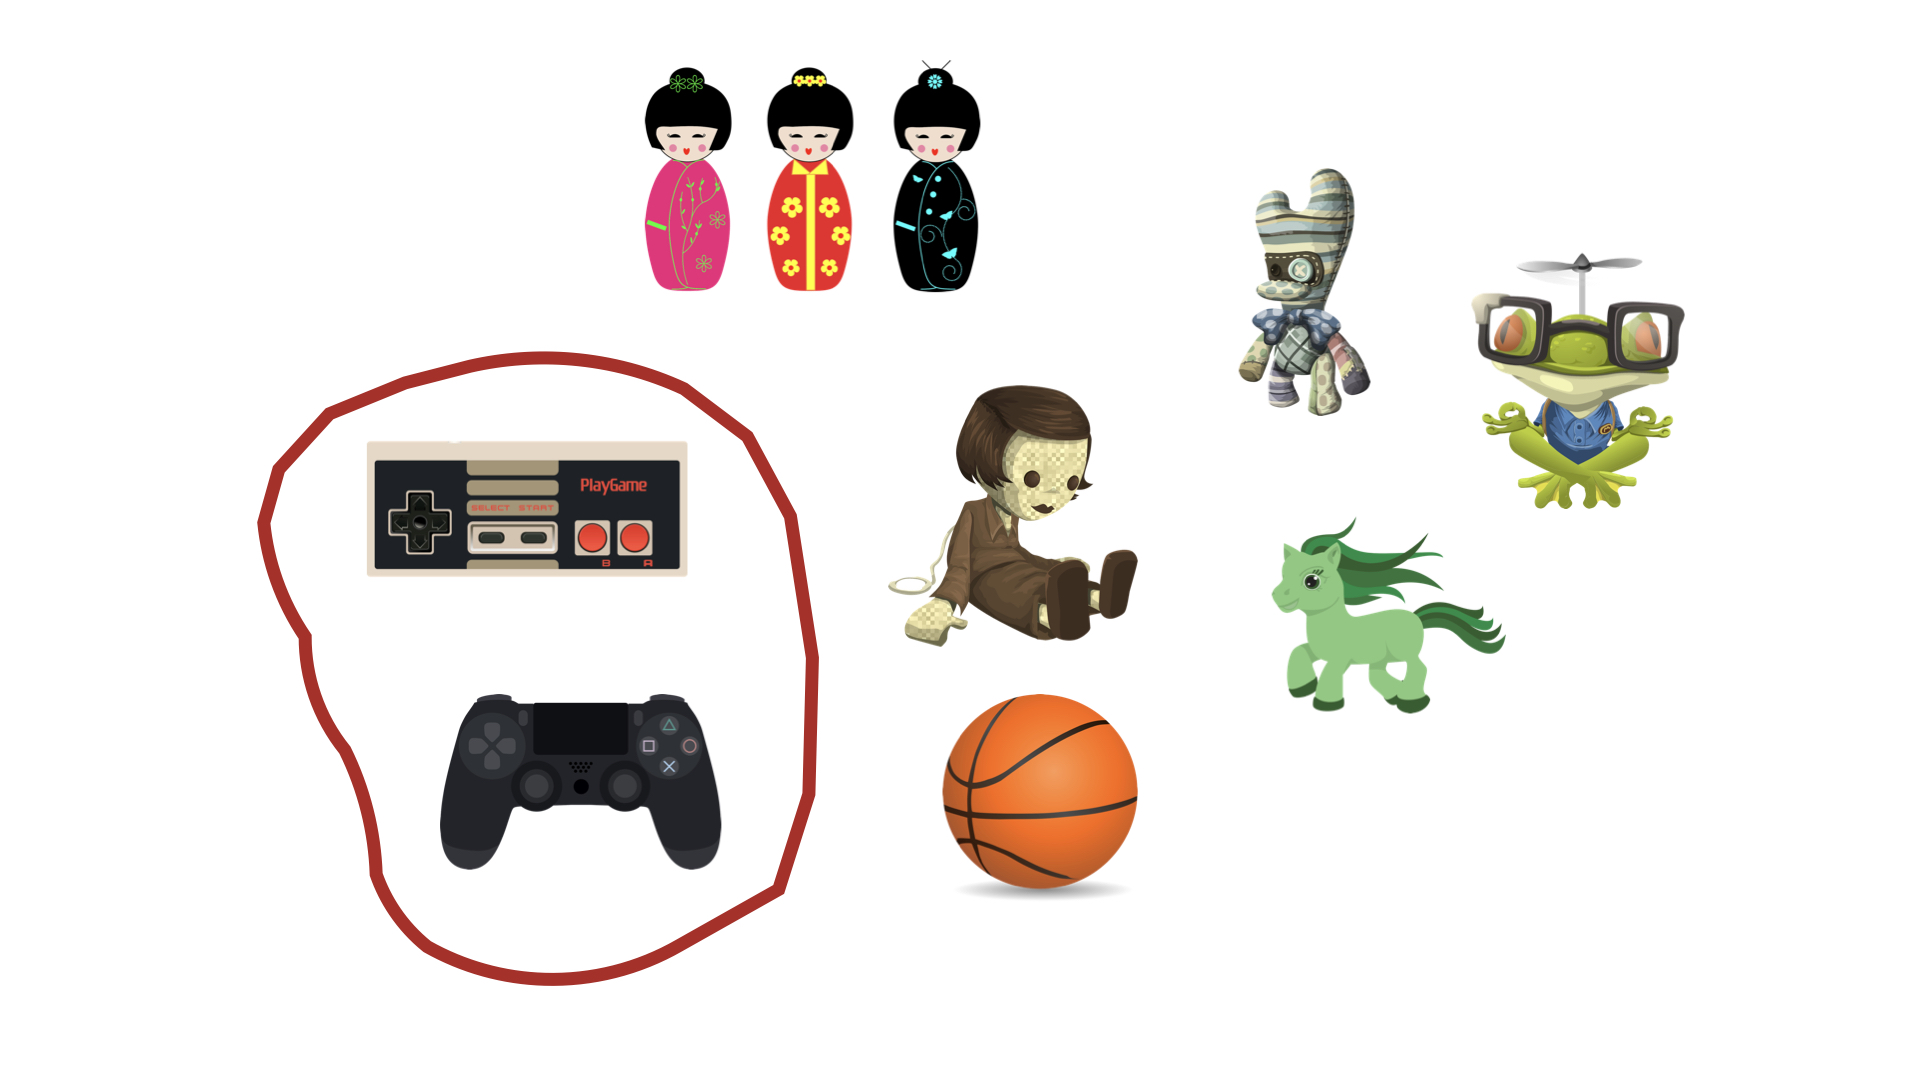
\includegraphics[width=\textwidth]{01a-sets-elements-cardinality/01a-sets-elements-cardinality-002.jpeg}
  \end{center}

\end{frame}

\begin{frame}
  \frametitle{Set}
  \framesubtitle{A collection of elements}

  \begin{center}
    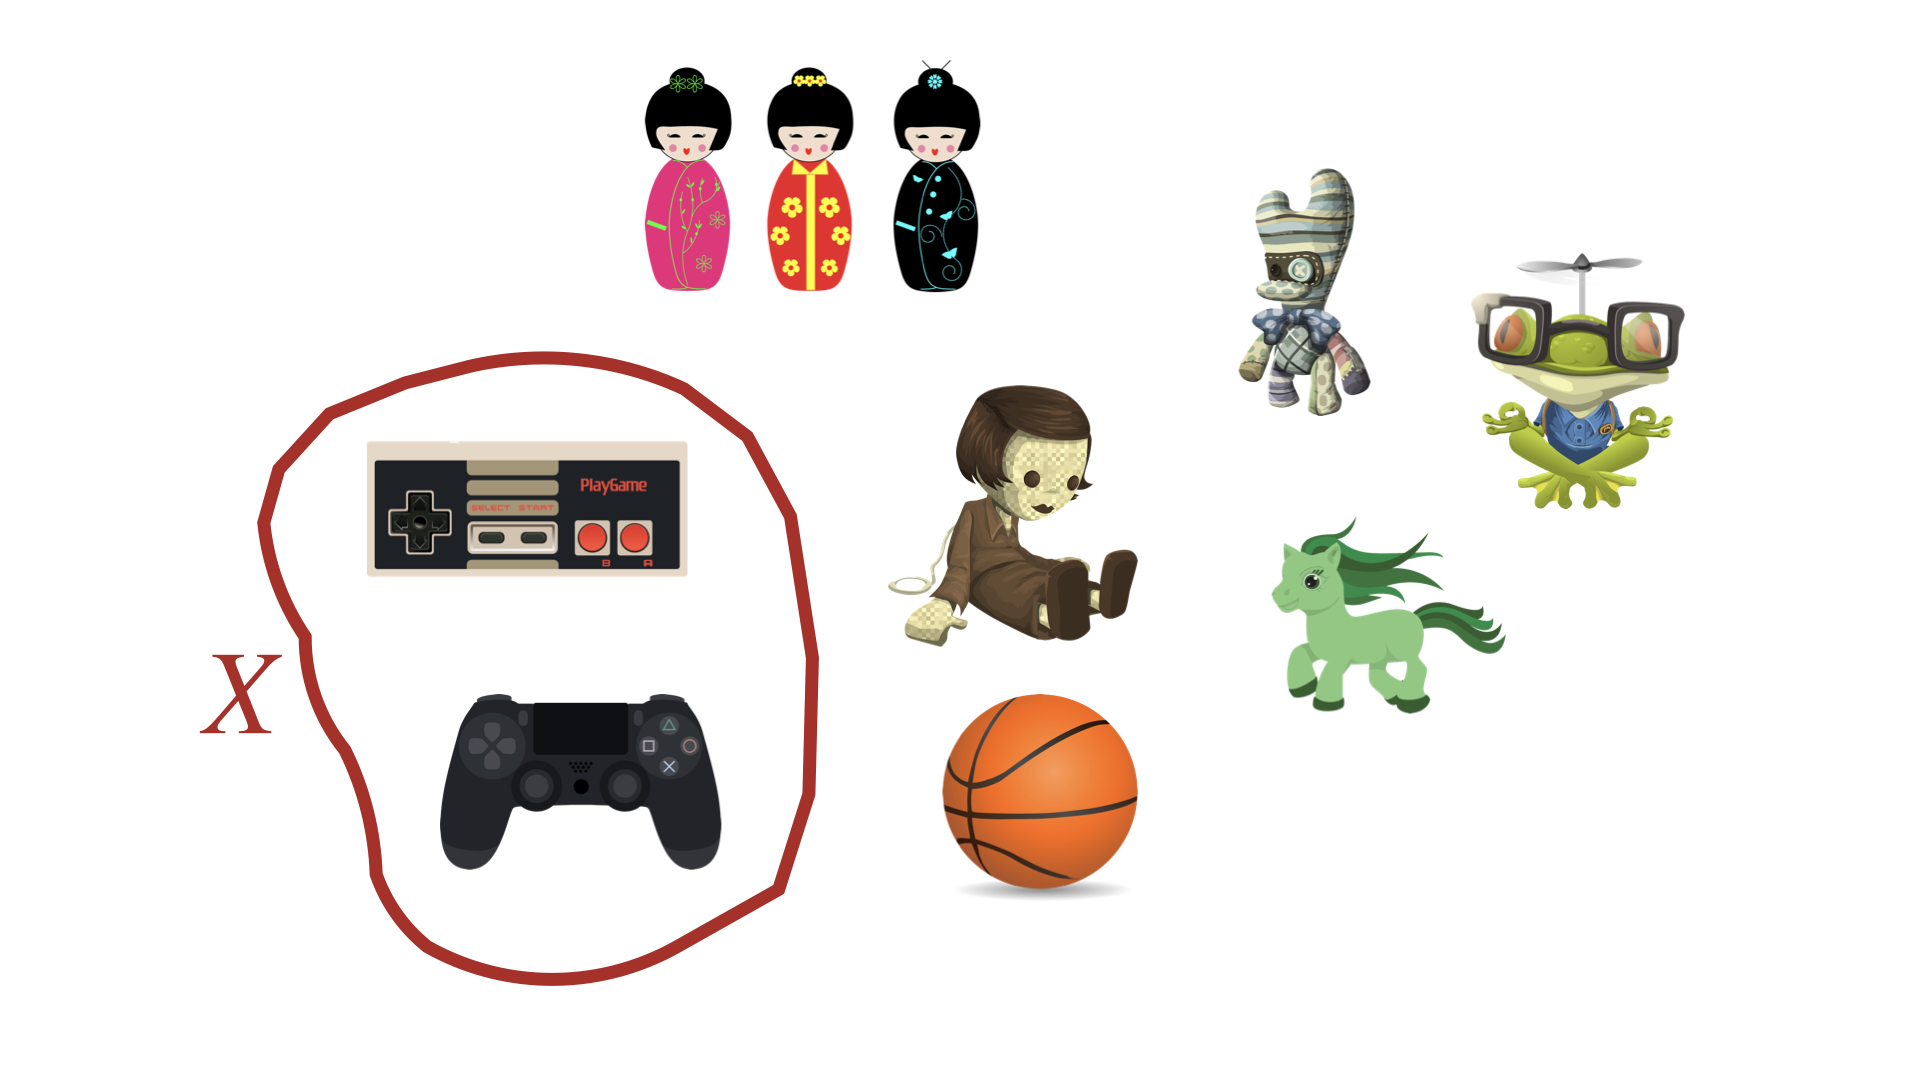
\includegraphics[width=\textwidth]{01a-sets-elements-cardinality/01a-sets-elements-cardinality-003.jpeg}
  \end{center}

\end{frame}

\begin{frame}
  \frametitle{Set}
  \framesubtitle{A collection of elements}
  \begin{minipage}{0.22\textwidth}
    \textbf{Notation}

    $X = \set{a,b}$

    $a \in X$

    $c \not \in X$

    \bigskip

    \textbf{Convention}

    $\set{a,b} = \set{b,a}$
  \end{minipage}
  \begin{minipage}{0.75\textwidth}\centering
    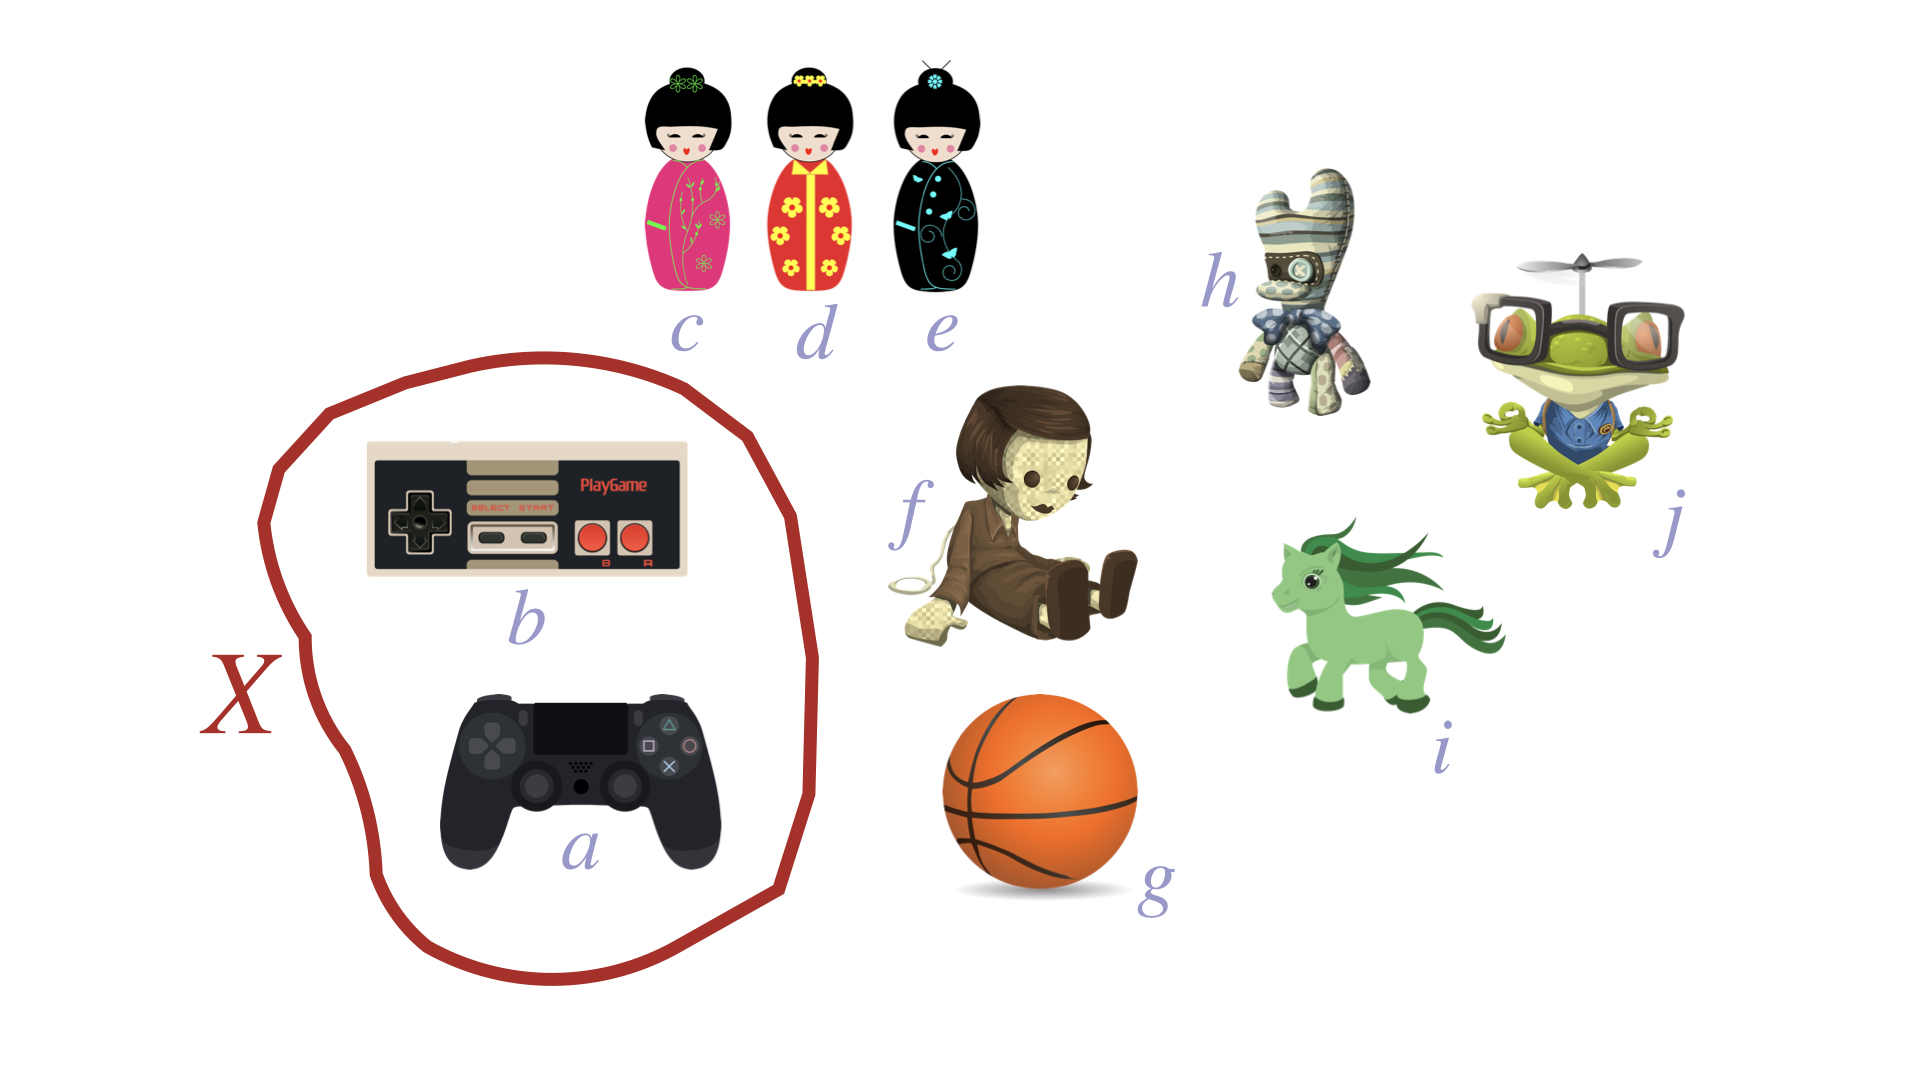
\includegraphics[width=\textwidth]{01a-sets-elements-cardinality/01a-sets-elements-cardinality-004.jpeg}
  \end{minipage}

\end{frame}

\begin{frame}

  \frametitle{Ways of describing or defining sets}

  \begin{minipage}{0.4\linewidth}
    \begin{enumerate}
      \item by listing elements
      \item by characteristic property
      \item by recursive definition
    \end{enumerate}
  \end{minipage}
  \begin{minipage}{0.55\linewidth}
  \end{minipage}

\end{frame}

\begin{frame}

  \frametitle{Ways of describing or defining sets}

  \begin{minipage}{0.4\linewidth}
    \begin{enumerate}
      \item \textbf{by listing elements}
      \item \mygray{by characteristic property}
      \item \mygray{by recursive definition}
    \end{enumerate}
  \end{minipage}
  \hfill
  \begin{minipage}{0.45\linewidth}

    $X = \set{0, 1, 2, 3, \dots}$

\bigskip

    $Y = \set{5, 7, 9, 11, \dots, 21}$
  \end{minipage}

\end{frame}


\begin{frame}

  \frametitle{Ways of describing or defining sets}

  \begin{minipage}{0.4\linewidth}
    \begin{enumerate}
      \item \mygray{by listing elements}
      \item \textbf{by characteristic property}
      \item \mygray{by recursive definition}
    \end{enumerate}
  \end{minipage}
  \hfill
  \begin{minipage}{0.45\linewidth}

    \begin{align*}
      X & = \set{x \in U \mid x \text{ is a game controler}} \\
      & = \set{a,b}
    \end{align*}

\bigskip

\begin{align*}
  Y &= \set{x \in X \mid x \text{ is retro}} \\
  & = \set{b}
\end{align*}
  \end{minipage}

\end{frame}

\begin{frame}

  \frametitle{Ways of describing or defining sets}

  \begin{minipage}{0.4\linewidth}
    \begin{enumerate}
      \item \mygray{by listing elements}
      \item \mygray{by characteristic property}
      \item \textbf{by recursive definition}
    \end{enumerate}
  \end{minipage}
  \hfill
  \begin{minipage}{0.45\linewidth}

    \textbf{Definition:}\\
    $\mathfrak{L}$ is a set of strings (symbols), such that
    \begin{enumerate}
      \item \textbf{anchor:} all natural numbers $\set{0, 1, 2, \dots}$ are part of $\mathfrak{L}$
      \item \textbf{step:} if $x, y \in \mathfrak{L}$, then so are the strings ``(x + y)'' and ``(x * y)''
      \item \textbf{exhaustion:} nothing else is in $\mathfrak{L}$
    \end{enumerate}

    \bigskip

\textbf{Examples:}
\begin{align*}
  5 &\in \mathfrak{L} \\
  3.5 &\not \in \mathfrak{L} \\
  ((4 * 2) + 3) &\in \mathfrak{L} \\
  (3 + 2 * 3) * 3 & \not \in \mathfrak{L} \\
\end{align*}
  \end{minipage}

\end{frame}

\begin{frame}
  \frametitle{Cardinality}
  \framesubtitle{Number of elements of a set}

  \begin{align*}
    X & = \set{a, b, c, d} \\
    \card{X} &= 4 && \text{\mygray{[finite set]}} \\ \noalign{\vskip20pt}
    Y &= \set{0, 1, 2, 3, \dots} \\
    \card{Y} &= \infty && \text{\mygray{[infinite set]}}
  \end{align*}

\end{frame}

\end{document}
